\section{Evaluation}
\label{sec:Evaluation}
This section is structured as, for each experiment and setup a detailed explanation and motivation on how and why the experiment is needed followed by the results of that experiment. The experiments are motivated by gathering as much information and results as possible to answer the research questions. The first subsection~\ref{sec:SD} will present the results from experiments with synthetic data where a reference image is available. The second subsection~\ref{sec:eval_spc} will present the result from images reconstructed from the SPC. No perfect reference image is available in those experiments therefore the images will be evaluated against near optimal image, no reference QA and against a state of the art SWIR camera. 



\subsection{Synthetic data}
\label{sec:SD}

\subsubsection{PSNR, SNR, SSIM}

\begin{figure}[H]
    \centering
    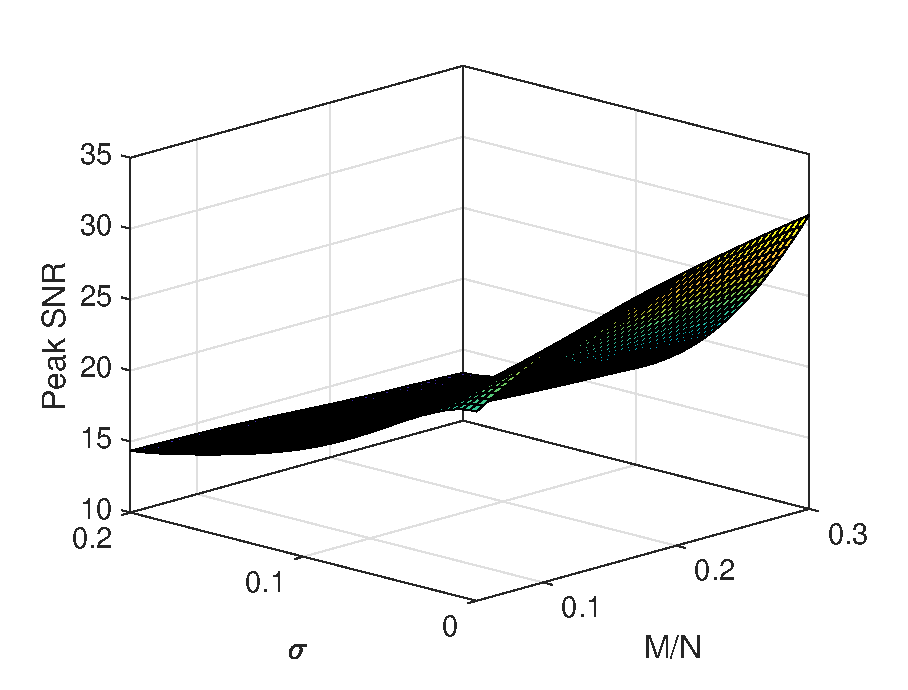
\includegraphics[width = 0.7\linewidth]{result/synt_sss/PSNR_fit.eps}
    \caption{Peak SNR result depending on number of measurements and simulated noise level.}
    \label{fig:psnr_3d}
\end{figure}

\begin{figure}[H]
    \centering
    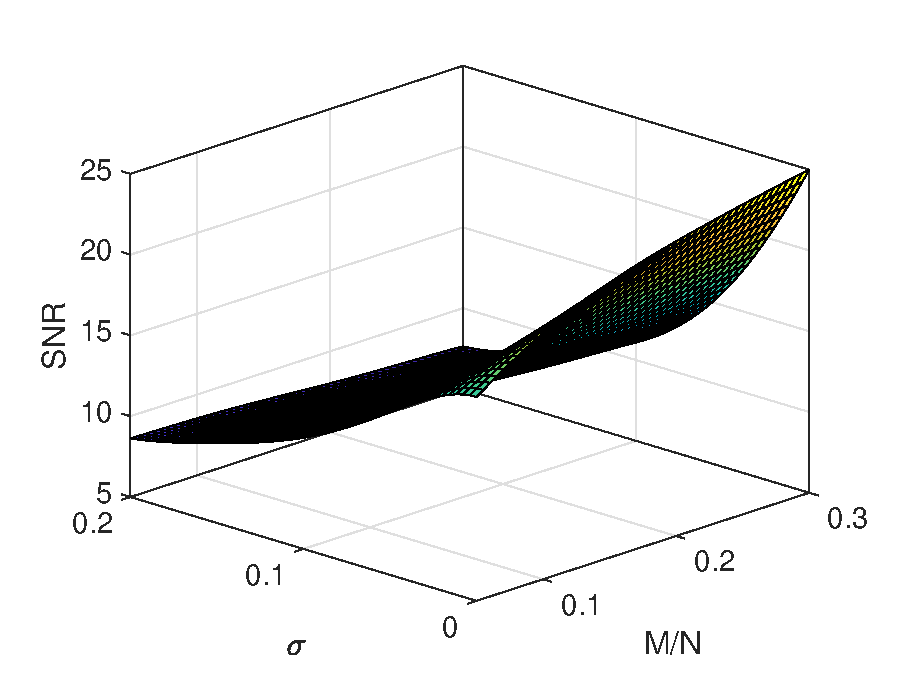
\includegraphics[width = 0.7\linewidth]{result/synt_sss/SNR_fit.eps}
    \caption{SNR result depending on number of measurements and simulated noise level.}
    \label{fig:snr_3d}
\end{figure}

\begin{figure}[H]
    \centering
    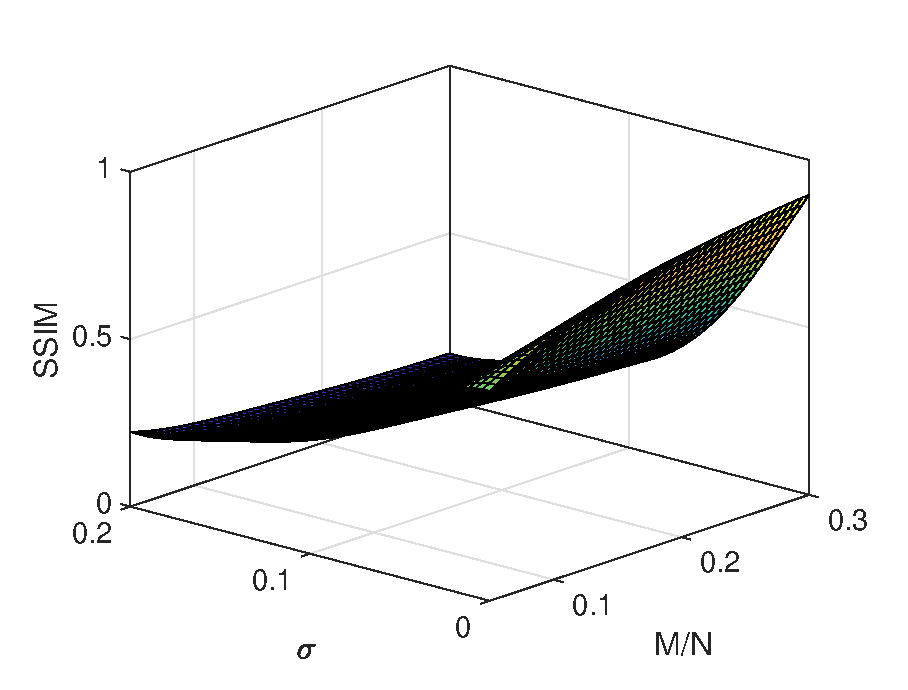
\includegraphics[width = 0.7\linewidth]{result/synt_sss/SSIM_fit.eps}
    \caption{SSIM result depending on number of measurements and simulated noise level.}
    \label{fig:snr_3d}
\end{figure}

\subsubsection{No Reference quality assessment}
BRISQUE lower score is better.

\begin{figure}[H]
    \centering
    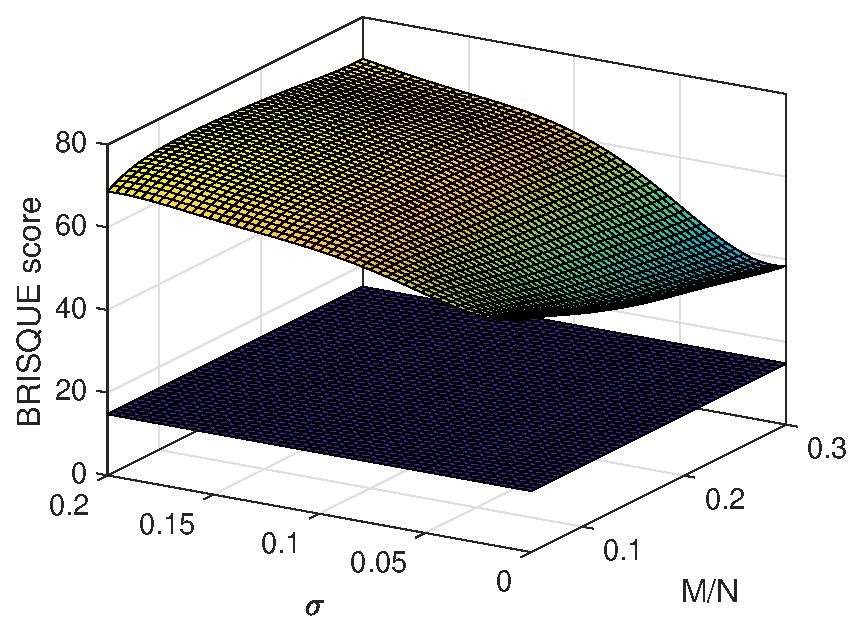
\includegraphics[width = 0.7\linewidth]{result/synt_brisque/BRISQUE_fit.eps}
    \caption{BRISQUE result depending on number of measurements and simulated noise level. Lower surface is reference image score.}
    \label{fig:Brisque_3d}
\end{figure}

\begin{figure}[H]
    \centering
    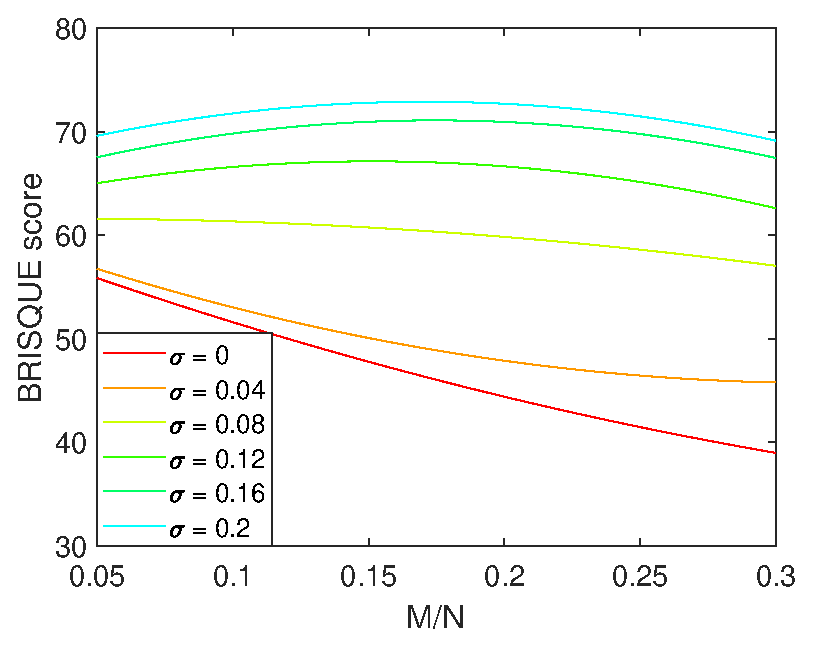
\includegraphics[width = 0.7\linewidth]{result/synt_brisque/Brisque_fit_flat.eps}
    \caption{BRISQUE result depending on number of measurements for different simulated noise levels.}
    \label{fig:Brisque_2d}
\end{figure}



\subsubsection{Dynamics in scene}
Dynamics in the scene can roughly be divided into three separate scenarios, in this section each of them will tested in a controlled environment with each scenario isolated to show how the signal and the reconstructed image is effected.\\[0.1in]

In the first scenario a object will be placed in an image but for each measurement matrix the location of the object will be moved in a bounded area of the image. This will model as a scene where the background is static but a person is standing in the same spot but moving around.

\begin{figure}[H]
    \centering
\begin{minipage}[t]{0.32\textwidth}
    
\includegraphics[width=1\textwidth]{result/dynamic/local/local_whole_time_org.png}
    \subcaption{Original reference image}
    \label{fig:local_1}
\end{minipage}
\begin{minipage}[t]{0.32\textwidth}
    
\includegraphics[width = \textwidth]{result/dynamic/local/local_whole_time_ref.png}
    \subcaption{Reconstructed $30\%$ image from reference image without movement}
    \label{fig:local_2}
\end{minipage}
\begin{minipage}[t]{0.32\textwidth}
    
\includegraphics[width = \textwidth]{result/dynamic/local/local_whole_time_res_psnr_29_snr_25_sssim_91.png}
    \subcaption{Reconstructed $30\%$ image with local movement}
    \label{fig:local_3}
\end{minipage}
    \caption{Local movement}
    \label{fig:local_dyn}
\end{figure}

The difference between figure~\ref{fig:local_2} and \ref{fig:local_3} is visible with the naked eye, not only does the object moving around get blurry and noisy but the whole image globally. In table~\ref{tab:local_dyn}...

\begin{table}[H]
    \centering
  \begin{tabular}{ | l | l | l |}
    \hline
    Peak SNR & SNR & SSIM \\ \hline
    29 & 25 & 91 \\ 
    \hline
  \end{tabular}
      \caption{Effects comparing non perturbed reconstructed image against reconstructed image with local movement}
    \label{tab:local_dyn}
\end{table}

Commenting the result from the table... In figure~\ref{fig:local_signal} the effects of the movement is shown plotted against the non perturbed signal.\\[0.1in]

\begin{figure}[H]
    \centering
\begin{minipage}[t]{0.495\textwidth}
    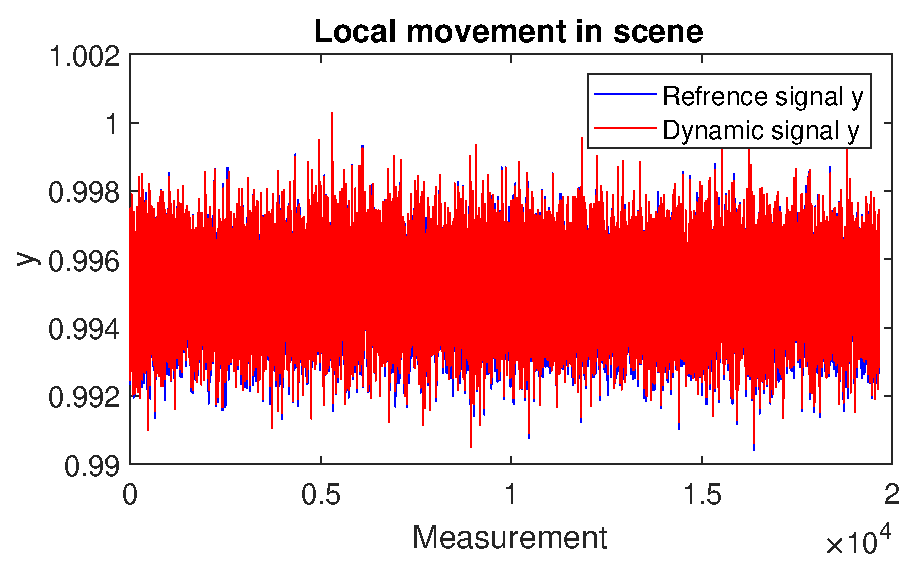
\includegraphics[width=1\textwidth]{result/dynamic/local/local_whole_time.eps}
    \subcaption{Signal.}
    \label{fig:local_sig_1}
\end{minipage}
\begin{minipage}[t]{0.495\textwidth}
    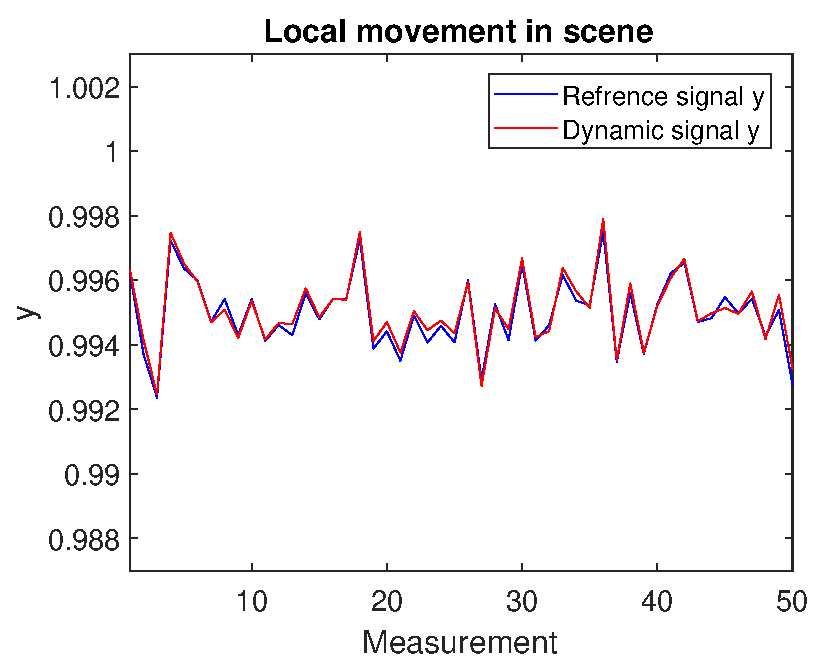
\includegraphics[width = \textwidth]{result/dynamic/local/local_whole_time_win.eps}
    \subcaption{Zoomed in view of the signal.}
    \label{fig:local_sig_2}
\end{minipage}
    \caption{Local movement, acquired signal}
    \label{fig:local_sig}
\end{figure}


As seen in figure~\ref{fig:local_sig_1} there is no obvious difference between the non perturbed reference signal and the distorted signal. In figure~\ref{fig:local_2} where some of the samples is displayed no large difference can be seen ether, the conclusion of this test implies that local movement in a scene will cause noise in the image globally and especially locally where the movement occurred. It also implies that local movement is very hard to detect on the signal even if a reference signal is available.\\[0.1in] 

%%%%%%%%%% Second scenario %%%%%%%%%%%%%%%%

The second scenario is an object is passing through, moves out or moves to an other place in the scene far from the original place. In other words, large global movement in the scene. The problem is modeled with a static background then as the simulated measurement is acquired the same object as in the first experiment will cross the scene, like a car,human or animal might do when using the SPC. The object will cross the scene in 1000 measurements of approximately 19000, corresponding to approximately $0.7$ seconds when capturing with the SPC in its current setup.



\begin{figure}[H]
    \centering
\begin{minipage}[t]{0.32\textwidth}
    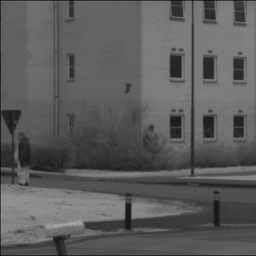
\includegraphics[width=1\textwidth]{result/dynamic/fly/flyby_1sec_org.png}
    \subcaption{Original reference image}
    \label{fig:fly_1}
\end{minipage}
\begin{minipage}[t]{0.32\textwidth}
    
\includegraphics[width = \textwidth]{result/dynamic/fly/flyby_1sec_ref.png}
    \subcaption{Reconstructed $30\%$ image from reference image without movement}
    \label{fig:fly_2}
\end{minipage}
\begin{minipage}[t]{0.32\textwidth}
    
\includegraphics[width = \textwidth]{result/dynamic/fly/flyby_1sec_res_psnr_23_snr_18_sssim_58.png}
    \subcaption{Reconstructed $30\%$ image with object passing trough}
    \label{fig:fly_3}
\end{minipage}
    \caption{Object passing trough scene.}
    \label{fig:fly_dyn}
\end{figure}

The difference between figure~\ref{fig:fly_2} and \ref{fig:fly_3} is visible with the naked eye, A global noise arises in the image and the object cant be seen. In table~\ref{tab:fly_dyn}...


\begin{table}[H]
    \centering
  \begin{tabular}{ | l | l | l |}
    \hline
    Peak SNR & SNR & SSIM \\ \hline
    23 & 18 & 58 \\ 
    \hline
  \end{tabular}
      \caption{Effects comparing non perturbed reconstructed image against reconstructed image with local movement}
    \label{tab:fly_dyn}
\end{table}


Commenting the result from the table... In figure~\ref{fig:fly_signal} the effects of the movement is shown plotted against the non perturbed signal.\\[0.1in]


\begin{figure}[H]
    \centering
\begin{minipage}[t]{0.495\textwidth}
    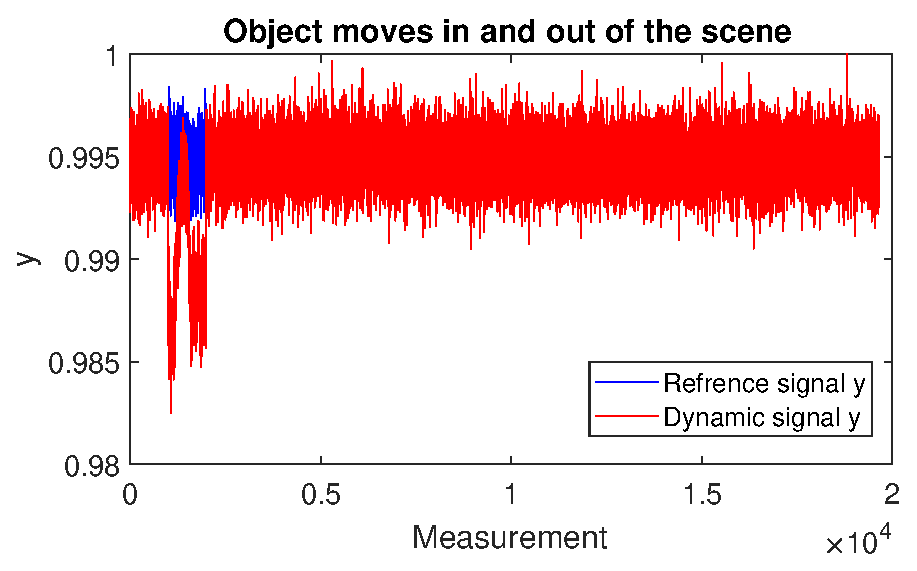
\includegraphics[width=1\textwidth]{result/dynamic/fly/flyby_sig.eps}
    \subcaption{Signal.}
    \label{fig:local_sig_1}
\end{minipage}
\begin{minipage}[t]{0.495\textwidth}
    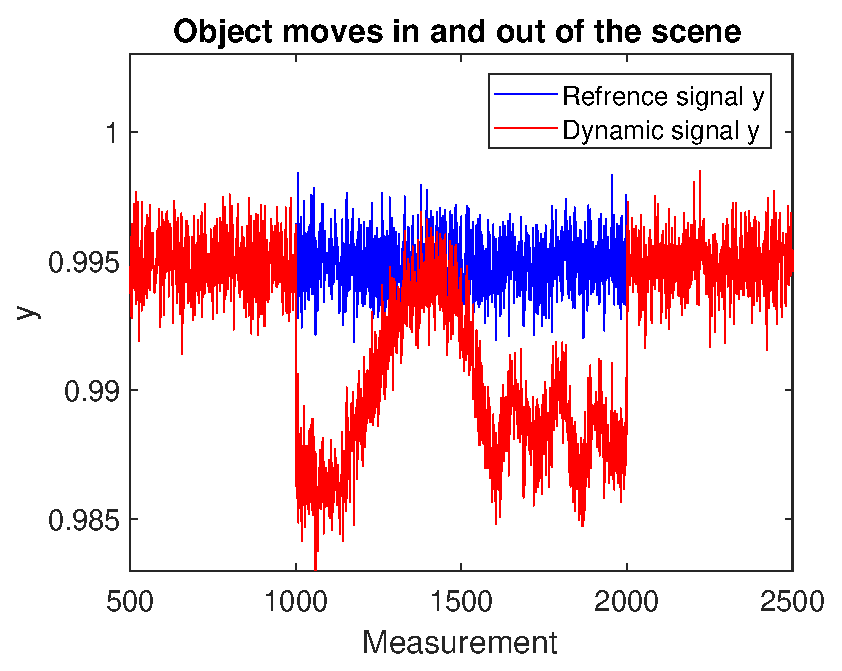
\includegraphics[width = \textwidth]{result/dynamic/fly/flyby_plot_win.eps}
    \subcaption{Zoomed in view of the signal.}
    \label{fig:local_sig_2}
\end{minipage}
    \caption{Global movement, acquired signal}
    \label{fig:local_sig}
\end{figure}

\begin{itemize}
    \item Large changes in the scene can be detected
    \item Remove the identified measurements to get a good signal 
\end{itemize}

%%%%%%%%%%%% Third %%%%%%%%%%%%%%%

The third scenario i luminance change in the scene caused by clouds occludes the sun or the light intensity from the lights is not constant. This scenario is modeled by adding or subtracting the global intensity in the image over the measurements. 

\begin{figure}[H]
    \centering
\begin{minipage}[t]{0.245\textwidth}
    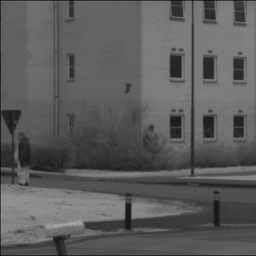
\includegraphics[width=1\textwidth]{result/dynamic/lum/intense_change_org.png}
    \subcaption{Original reference image}
    \label{fig:lum_1}
\end{minipage}
\begin{minipage}[t]{0.245\textwidth}
    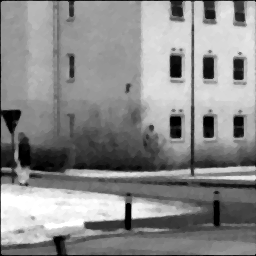
\includegraphics[width = \textwidth]{result/dynamic/lum/intense_change.png}
    \subcaption{Reconstructed $30\%$ image from reference image without movement}
    \label{fig:lum_2}
\end{minipage}
\begin{minipage}[t]{0.245\textwidth}
    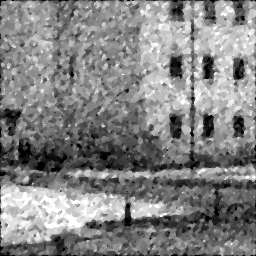
\includegraphics[width = \textwidth]{result/dynamic/lum/intense_change_psnr_19_snr_14_sssim_38.png}
    \subcaption{Reconstructed $30\%$ image with global luminance change}
    \label{fig:lum_3}
\end{minipage}
\begin{minipage}[t]{0.245\textwidth}
    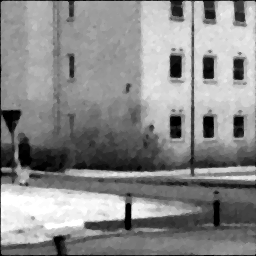
\includegraphics[width = \textwidth]{result/dynamic/lum/intense_change_movemean_psnr_33_snr_29_sssim_93.png}
    \subcaption{Reconstructed $30\%$ image with mean subtraction}
    \label{fig:lum_4}
\end{minipage}
    \caption{Global luminance change in scene.}
    \label{fig:lum_dyn}
\end{figure}


The difference between figure~\ref{fig:lum_2} and \ref{fig:lum_3} is visible with the naked eye, A global noise arises in the image, but as seen in figure~\ref{fig:lum_4} the effect can be suppressed explained under figure~\ref{fig:lum_sig}. In table~\ref{tab:fly_dyn}...


\begin{table}[H]
    \centering
  \begin{tabular}{ | l | l | l | l |}
    \hline
     & Peak SNR & SNR & SSIM \\ \hline
    Perturbed signal & 19 & 14 & 38 \\ \hline
    Mean subtracted signal & 33 & 29 & 93 \\
    \hline
  \end{tabular}
      \caption{Effects comparing non perturbed reconstructed image against reconstructed image with global luminance change}
    \label{tab:lum_dyn}
\end{table}


Commenting the result from the table... In figure~\ref{fig:lum_signal} the effects of global luminance is shown plotted against the non perturbed signal.\\[0.1in]


\begin{figure}[H]
    \centering
\begin{minipage}[t]{0.495\textwidth}
    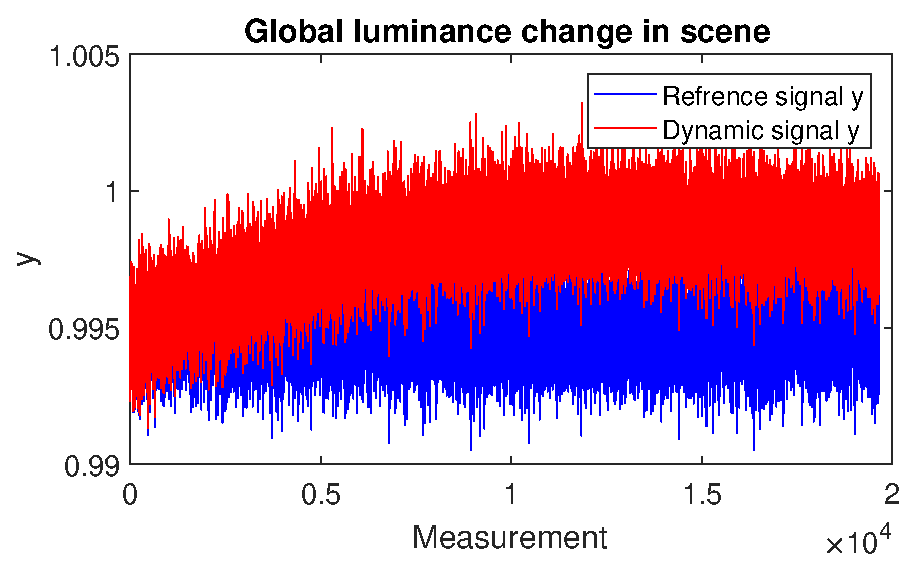
\includegraphics[width=1\textwidth]{result/dynamic/lum/intense_change.eps}
    \subcaption{Signal.}
    \label{fig:lum_sig_1}
\end{minipage}
\begin{minipage}[t]{0.495\textwidth}
    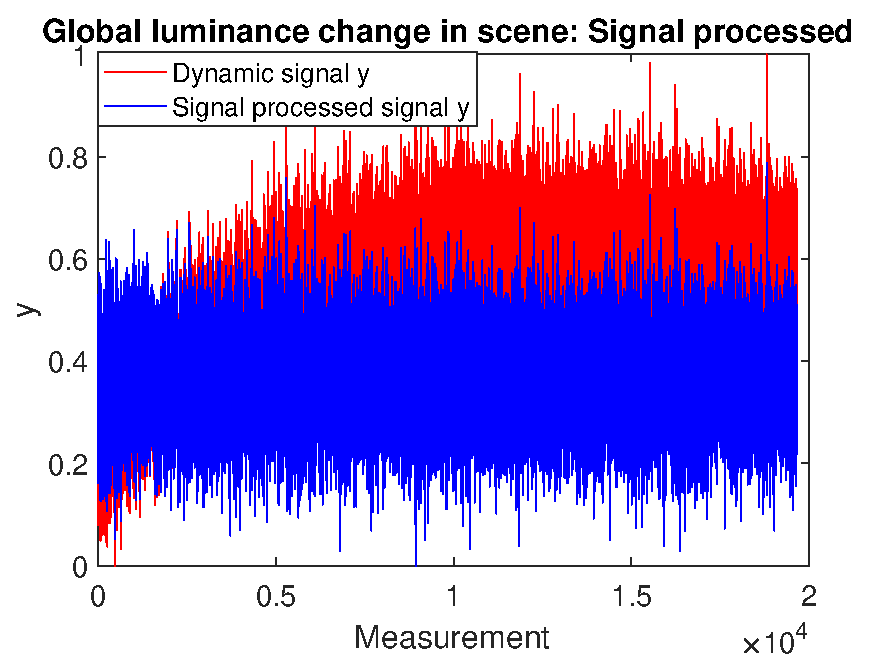
\includegraphics[width = \textwidth]{result/dynamic/lum/intense_change_sp.eps}
    \subcaption{Zoomed in view of the signal.}
    \label{fig:lum_sig_2}
\end{minipage}
\begin{minipage}[t]{0.495\textwidth}
    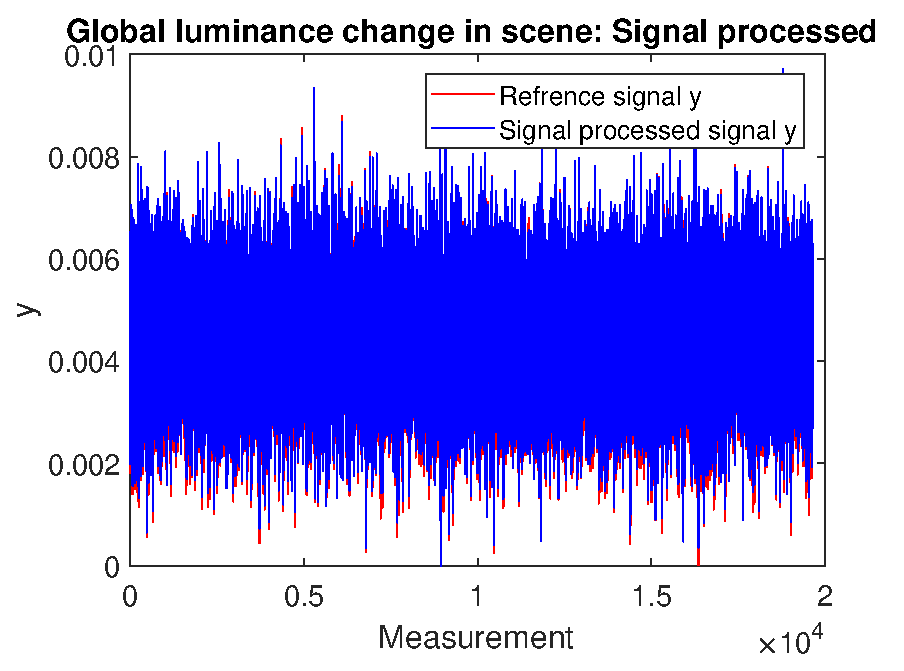
\includegraphics[width=1\textwidth]{result/dynamic/lum/intense_change_sp_ref.eps}
    \subcaption{Signal.}
    \label{fig:lum_sig_3}
\end{minipage}
\begin{minipage}[t]{0.495\textwidth}
    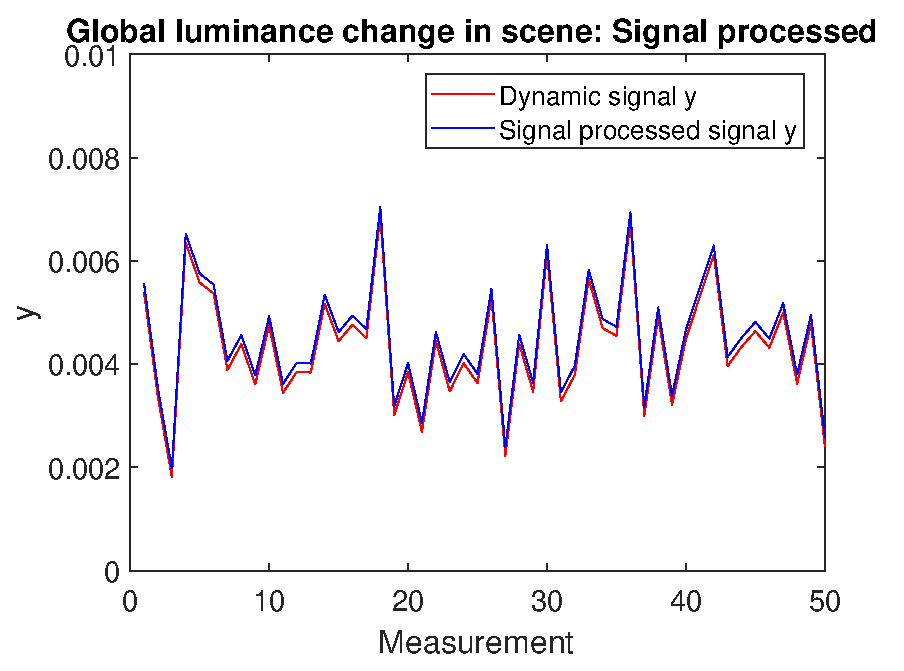
\includegraphics[width = \textwidth]{result/dynamic/lum/intense_change_sp_ref_win.eps}
    \subcaption{Zoomed in view of the signal.}
    \label{fig:lum_sig_4}
\end{minipage}
    \caption{Global movement, acquired signal}
    \label{fig:lum_sig}
\end{figure}

\begin{itemize}
    \item Dynamic signal v. Reference signal
    \item Dynamic signal v. Mean subtracted signal
    \item Reference signal v. Mean subtracted signal
    \item Comment on the window, pretty good.
    \item Can be detected with the knowledge that the signal should be stationary. Signal process the signal to look like a stationary signal.
\end{itemize}

\subsection{SPC evaluation}
\label{sec:eval_spc}

\subsubsection{Soft chessboard}
\todo[inline]{Todo: Skapa rekonstruerade bilder från homagraphin och jämnför de rekonstruerade med referensbilden}
This evaluation is designed to confirm that the images reconstructed by the SPC follows the same characteristics as the reconstruction of the synthetic data.

\begin{figure}[H]
    \centering
    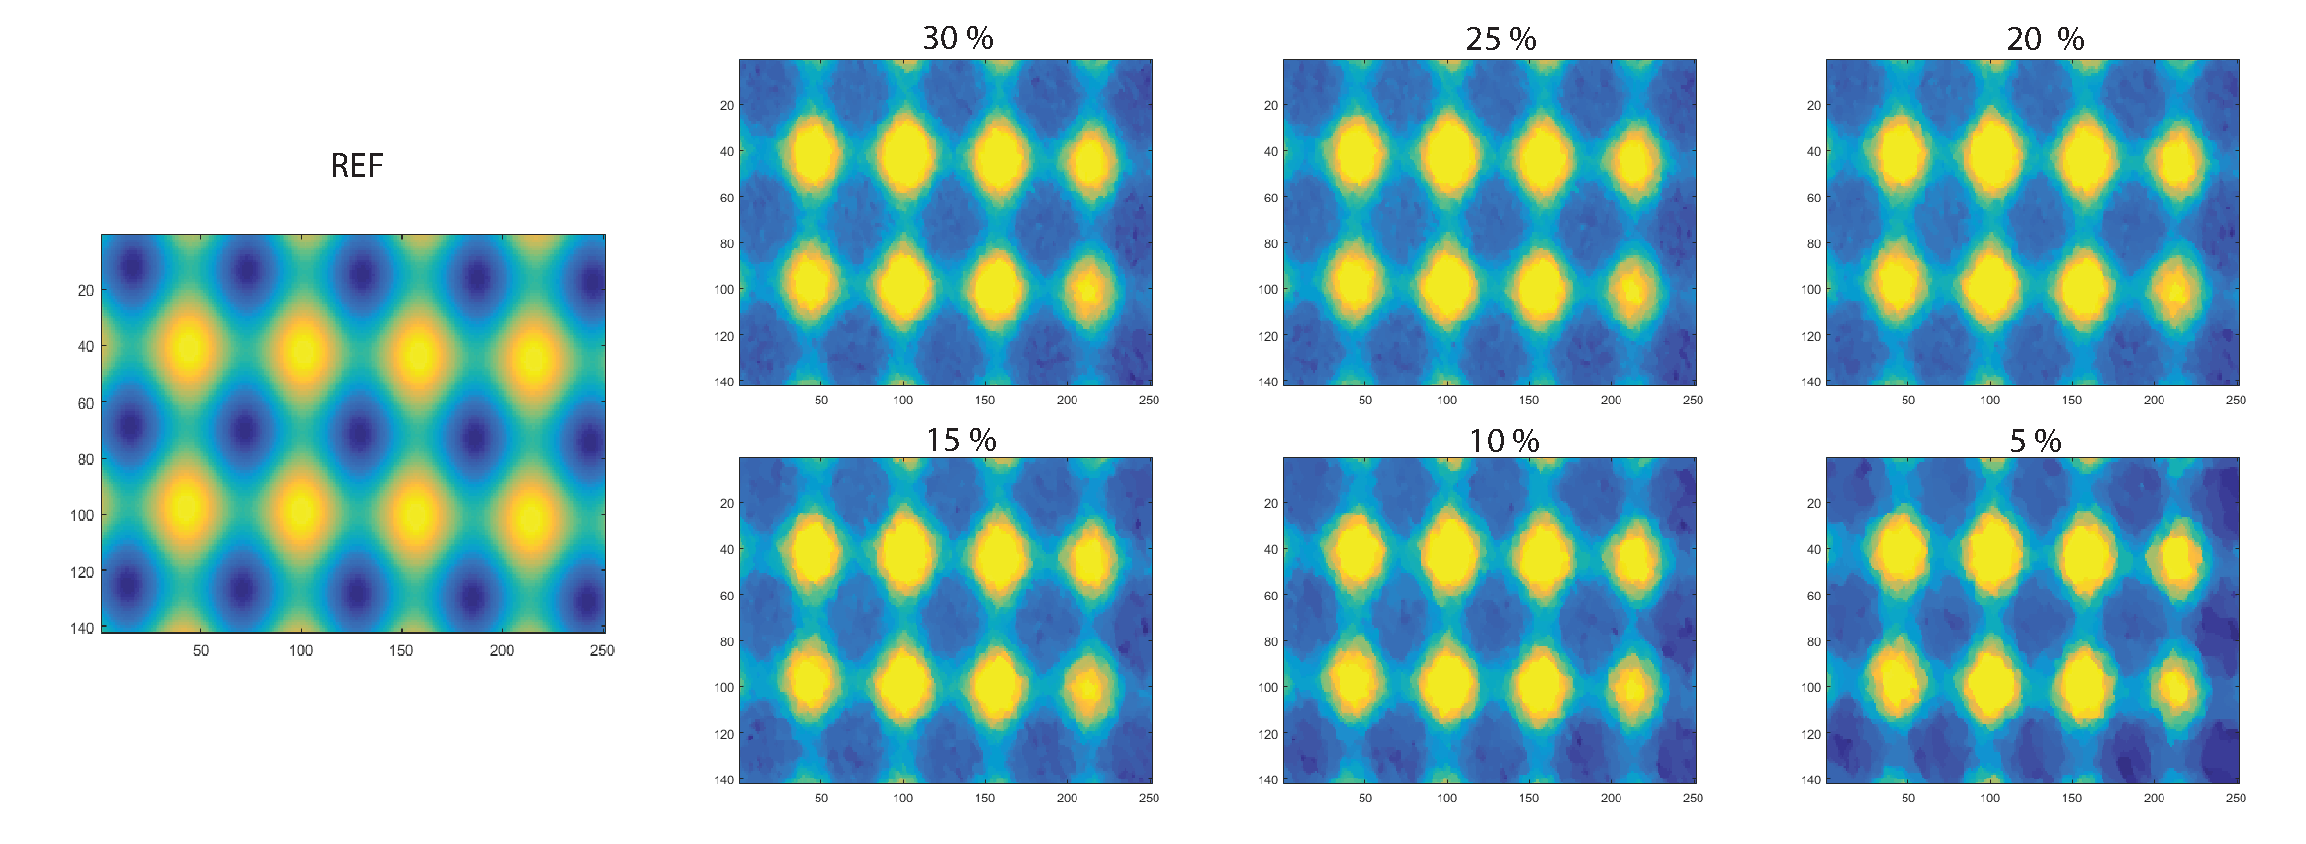
\includegraphics[width=1\linewidth]{result/homo/Hom_im.eps}
    \caption{The reconstructed images with different number of measurements and the reference image transformed to fit the SPC images using homography.}
    \label{fig:hom_over_im}
\end{figure}

\begin{figure}[H]
    \centering
\begin{minipage}[t]{0.49\textwidth}
    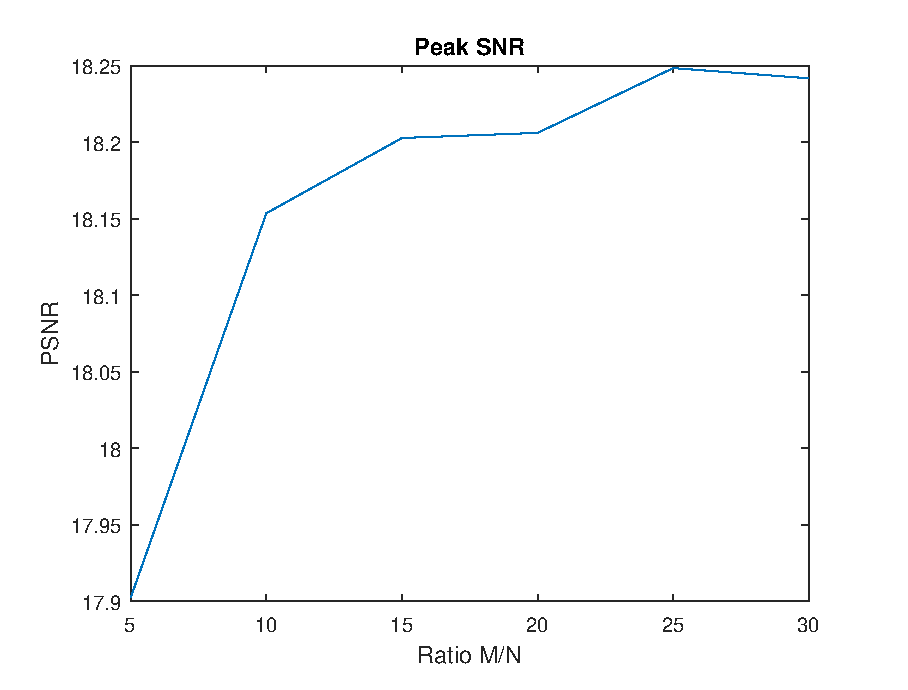
\includegraphics[width=1\textwidth]{result/homo/hom_PSNR.eps}
    \subcaption{Peak SNR for reconstructed images against reference image.}
    \label{fig:hom_psnr}
\end{minipage}
\begin{minipage}[t]{0.49\textwidth}
    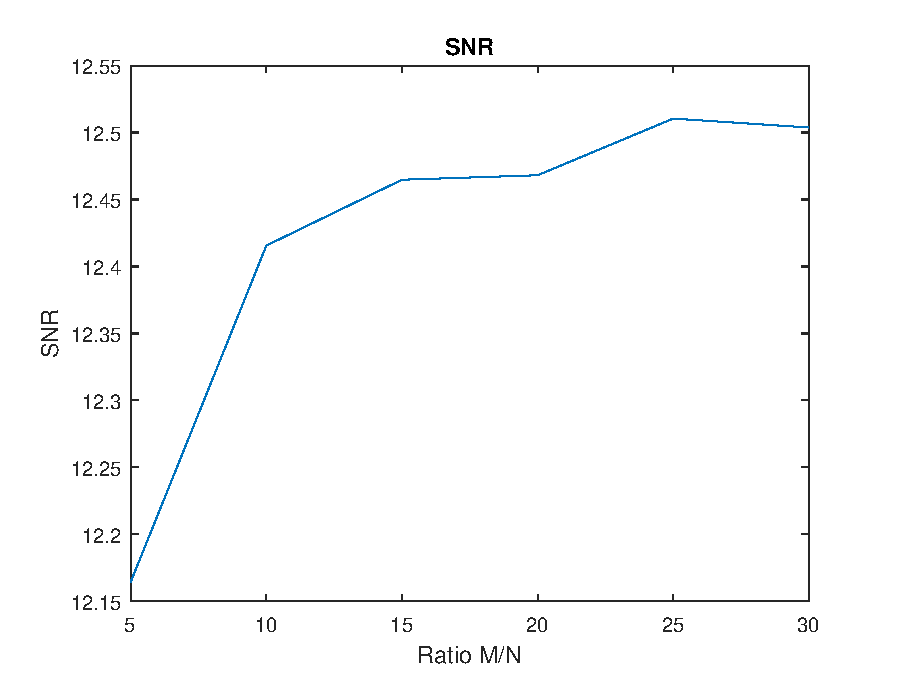
\includegraphics[width = \textwidth]{result/homo/hom_SNR.eps}
    \subcaption{SNR for reconstructed images against reference image.}
    \label{fig:hom_snr}
\end{minipage}
\begin{minipage}[t]{0.49\textwidth}
    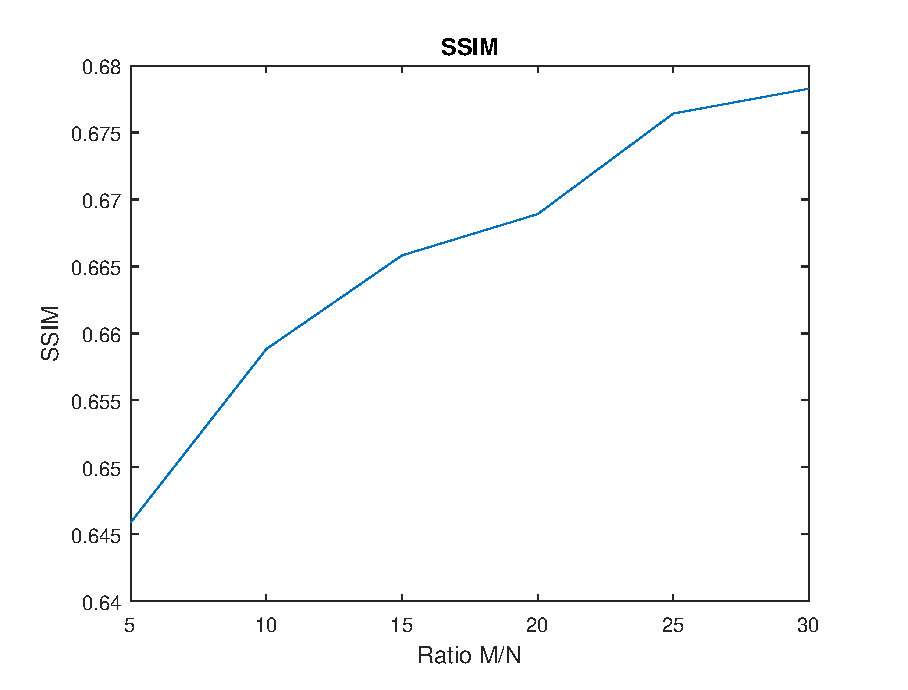
\includegraphics[width=1\textwidth]{result/homo/hom_SSIM.eps}
    \subcaption{SSIM score for reconstructed images against reference image.}
    \label{fig:hom_ssim}
\end{minipage}
    \caption{Signal quality of SPC images compared to reference image}
    \label{fig:hom_score}
\end{figure}


\subsubsection{No reference quality assessment}
Using the no reference quality assessment measurement BRISQUE to evaluate the SPC images. Each image is evaluated at reconstruction rate $5\%$ to $30\%$.

\begin{figure}[H]
    \centering
    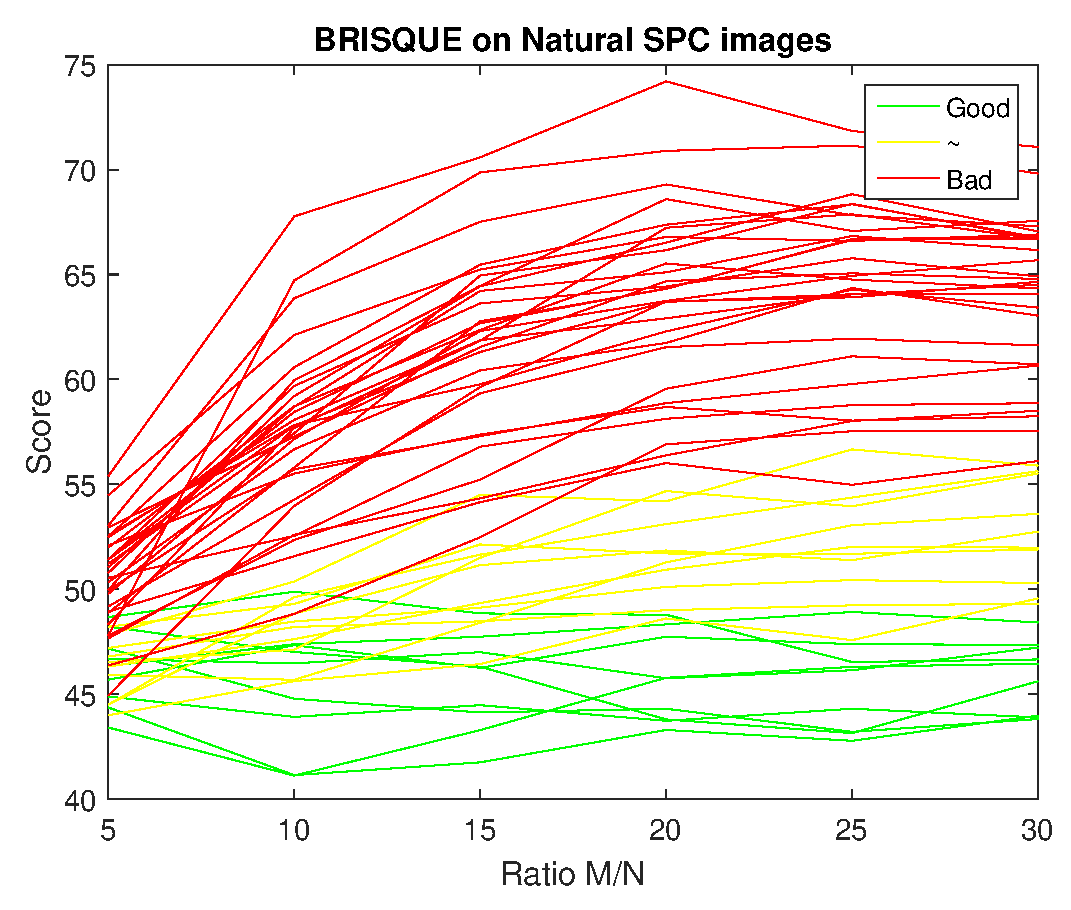
\includegraphics[width = 0.7\linewidth]{result/SPC_NRQA/plot.eps}
    \caption{BRISQUE result.}
    \label{fig:brisque_plot}
\end{figure}

\begin{figure}[H]
    \centering
    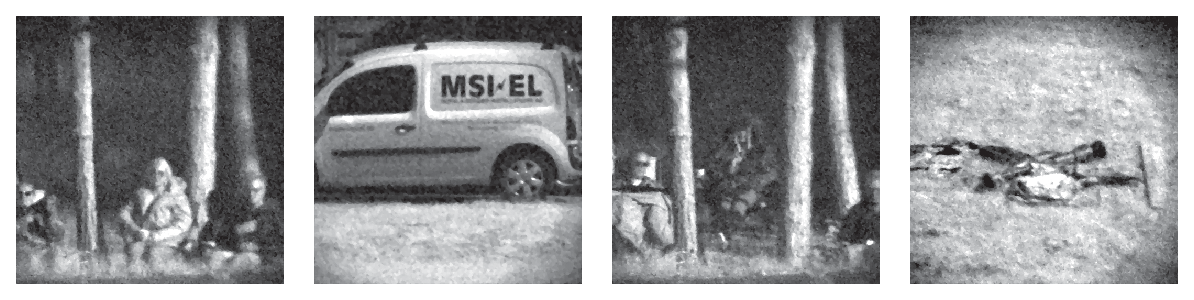
\includegraphics[width = 1\linewidth]{result/SPC_NRQA/good.eps}
    \caption{Example of 'good' images corresponding to the green lines in figure~\ref{fig:brisque_plot}.}
    \label{fig:good_plot}
\end{figure}

\begin{figure}[H]
    \centering
    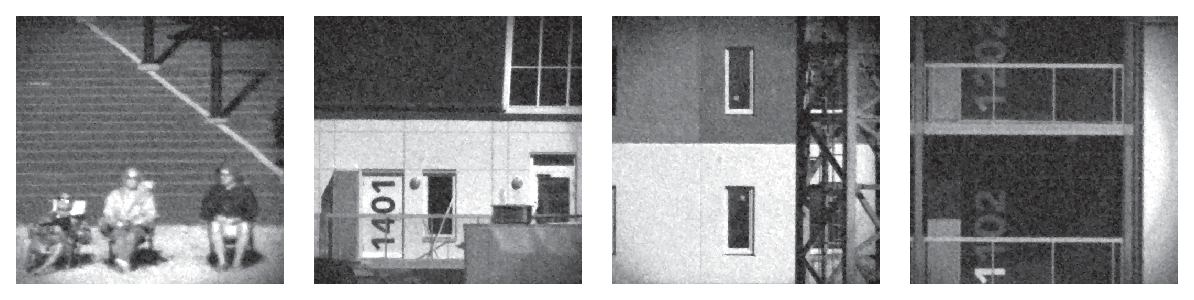
\includegraphics[width = 1\linewidth]{result/SPC_NRQA/half.eps}
    \caption{Example of 'medium good' images corresponding to the yellow lines in figure~\ref{fig:brisque_plot}.}
    \label{fig:half_plot}
\end{figure}

\begin{figure}[H]
    \centering
    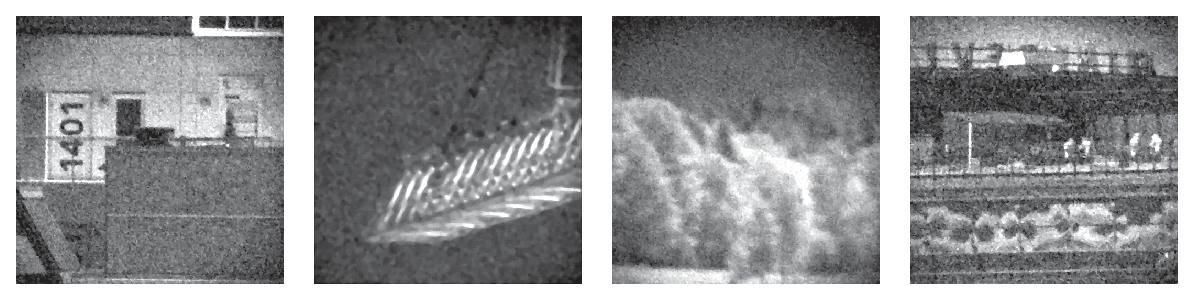
\includegraphics[width = 1\linewidth]{result/SPC_NRQA/bad.eps}
    \caption{Example of 'bad' images corresponding to the red lines in figure~\ref{fig:brisque_plot}.}
    \label{fig:bad_plot}
\end{figure}

\begin{itemize}
    \item Good images are:
    \item Medium good images are:
    \item Bad images are:
\end{itemize}


\subsubsection{Modulation Transfer Function}
The MTF is used to comparing the sharpness of cameras and lenses.  

%for two reasons: (1) Image contrast is half its low frequency or peak values,hence detail is still quite visible. The eye is relatively insensitive to detail at spatial frequencies where MTF is low: 10 or less. (2) The response of most cameras falls off rapidly in the vicinity of MTF50 and MTF50P. MTF50P is a better metric for strongly sharpened cameras that have “halos” near edges and corresponding peaks in their MTF response.

The MTF from the SPC is compared to a state of the art SWIR camera. Two scenes was captured by the SPC and a conventional SWIR camera containing printed sheath of paper with simple tilted shapes on them, see figure~\ref{fig:mtf_target}. 



\begin{figure}[H]
    \centering
    
\includegraphics[width=0.9\linewidth]{result/mtf/Target.eps}
    \caption{Printed targets with markings where the MTF measurements was performed}
    \label{fig:mtf_target}
\end{figure}

In the resulting images MTF measurements was performed on the specified edges to gather a mean and standard deviation for each camera. For the SPC, images reconstructed from 5\% to 30\% was tested in order to see if the number of measurements effected the MTF result. In figure~\ref{fig:mtf_target_im} the images from the SWIR camera and SPC are presented.

\begin{figure}[H]
    \centering
    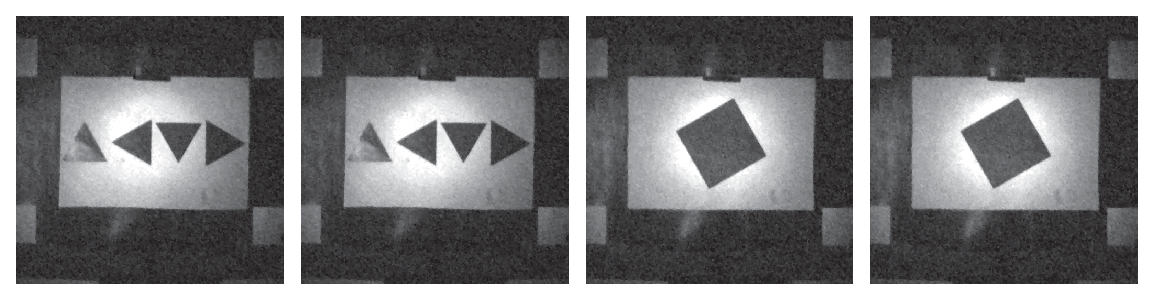
\includegraphics[width=1\linewidth]{result/mtf/Target_im.eps}
    \caption{SPC and state of the art SWIR camera output images. (OBS! Bilder från Raptorn ska läggas till)}
    \label{fig:mtf_target_im}
\end{figure}


\subsection{MTF}


\begin{figure}[H]
    \centering
    \begin{minipage}{0.49\textwidth}
    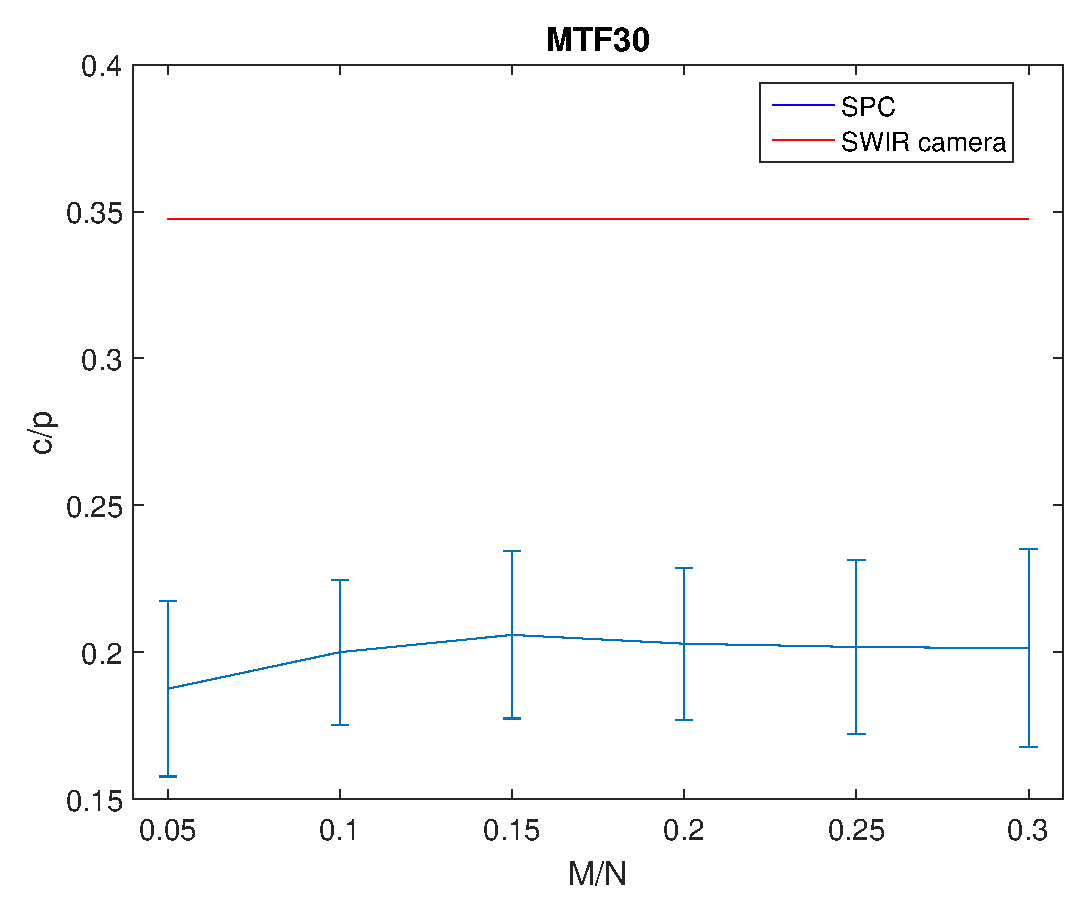
\includegraphics[width=1\textwidth]{result/mtf/mtf30.eps}
    \subcaption{MTF30 result.}
    \label{fig:mtf30}
\end{minipage}
\begin{minipage}{0.49\textwidth}
    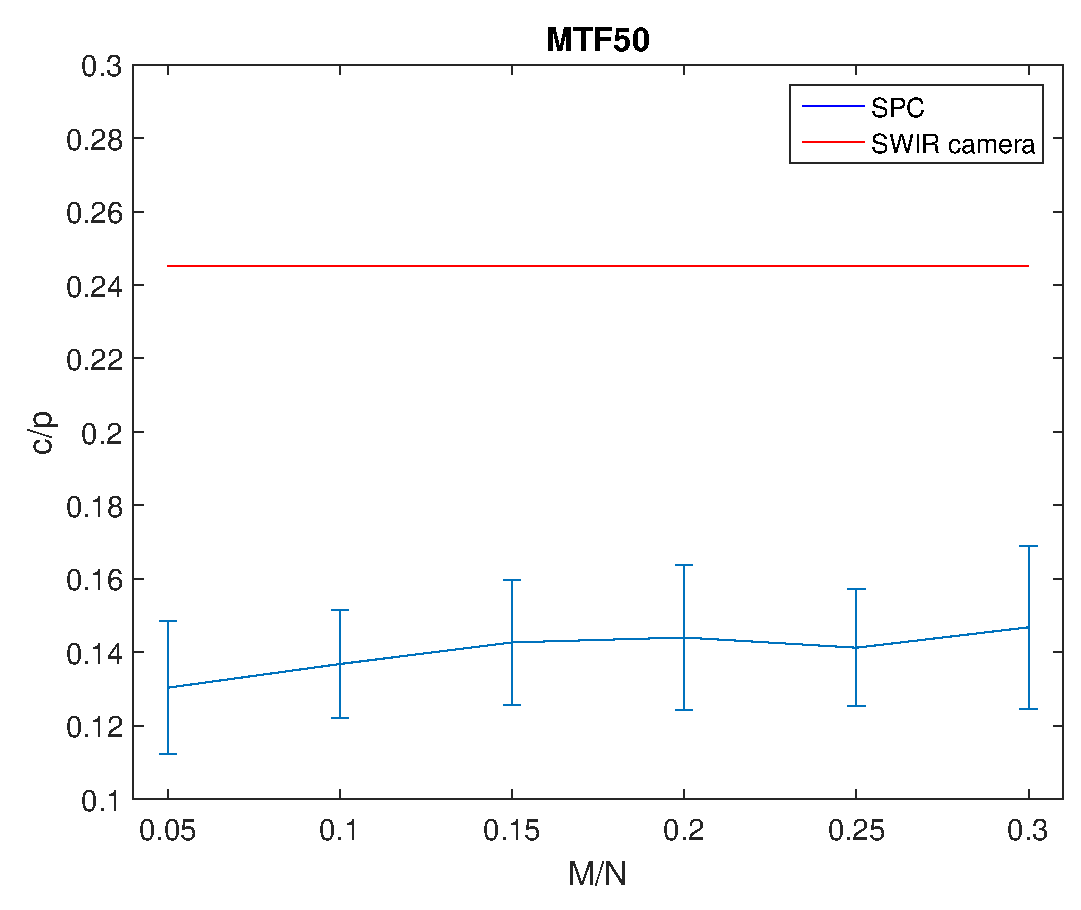
\includegraphics[width = \textwidth]{result/mtf/mtf50.eps}
    \subcaption{MTF50 result.}
    \label{fig:i2}
\end{minipage}
    \caption{MTF results. (OBS! inte rätt figurer)}
    \label{fig:mtf50}
\end{figure}

\subsection{Edge response}
The edge response is measured in the distance (pixels) required for the edge to rise from $10\%$ to $90\%$. In figure~\ref{fig:rise} the result from the experiment in presented. 

\begin{figure}[H]
    \centering
    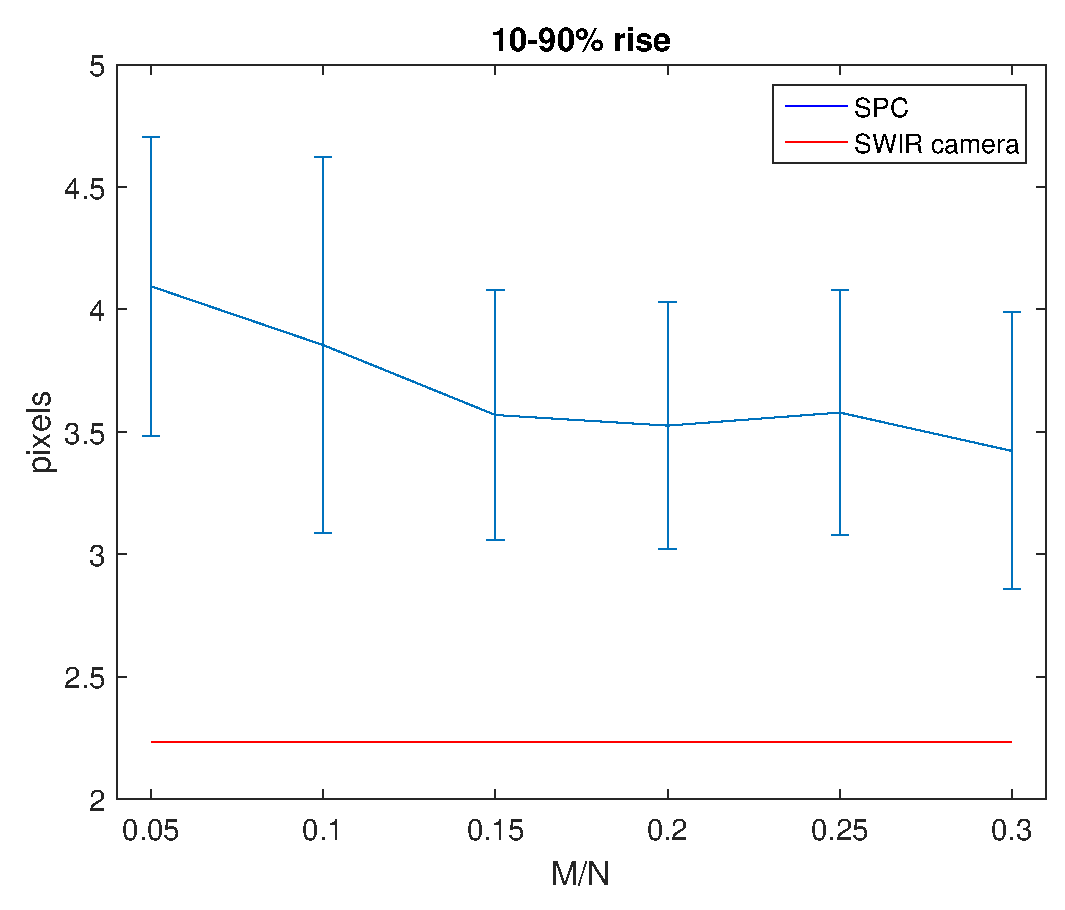
\includegraphics[width=0.5\linewidth]{result/mtf/10-90_rise.eps}
    \caption{10-90\% rise in pixels. (OBS! inte rätt figur)}
    \label{fig:rise}
\end{figure}






